\documentclass{article}
\usepackage[utf8]{inputenc}
\usepackage{graphicx} % Required for inserting images
\usepackage{float}    % For [H] specifier
\usepackage{caption}  % Better captions
\usepackage{geometry} % Optional: better page margins
\usepackage{subcaption} % For subfigures
\usepackage{amssymb}
\geometry{margin=1in}


\title{}
\author{}
\date{}

\begin{document}


\section*{Theoretical Questions}
\bigskip
\subsection*{Question 2}
\bigskip

\subsubsection*{\boldmath a) Justification for $p_L < c + c_S$}
\noindent
When the \emph{Vilnius} bakery has unsold surplus product, it has a deal with a local feed mill that purchases the surplus at a lower price, denoted as $p_L$. 
In practice, this price should be lower than the sum of the shipping costs and the production costs denoted as $c + c_S$, because otherwise it would create an incentive for the bakery to overproduce on purpose in order to generate more profit when trading with the animal feed producer. In the situation where $p_L \geq c + c_S$, the business model would deem the business model of a bakery entirely unoptimal. This is because distributing the product between customers would generate less profit or the same amount of profit as simply selling it to the feed producer. This ensures that $p_L < c + c_S$ keeps customer sales profitable while allowing the feed mill to function as a mean to minimize losses.

\subsubsection*{\boldmath b) Adding $p_L$ and $c_S$ to the profit function}
\noindent 
To incorporate the $p_L$ %(clearance price) 
and the $c_S$, %(shipping cost)
 we will modify the classical profit function:

\[
\Pi(Q, Y; c, p) = p \cdot \min\{Q, Y\} - c \cdot Q
\]
\noindent
If we now include clearance sales, where we have $Q - Y$ unsold units, if $Q > Y$. Then these are sold at price $p_L$, and the costs of shipping them are $c_S$ per unit, then our profit function becomes:

\[
\Pi(Q, Y; c, p, p_L, c_S) = p \cdot \min\{Q, Y\} + (p_L - c_S) \cdot (Q - Y)^+ - c \cdot Q,
\]
\noindent
where $(Q - Y)^+ = \max(Q - Y, 0)$ denotes the number of surplus units.


\noindent
\\We want to simplify the form to match:

\[
\Pi(Q, Y; \tilde{c}, \tilde{p}) = \tilde{p} \cdot \min\{Q, Y\} - \tilde{c} \cdot Q,
\]
\noindent
where $\tilde{p}$ and $\tilde{c}$ represent adjusted effective values. In this setup, we define:

\[
\tilde{p} = p, \quad \tilde{c} = c - (p_L - c_S) \cdot \mathbb{P}(Q > Y).
\]

\noindent
The term $\tilde{c}$ is the effective cost per unit, reduced by the expected value recovered from the sale of surplus goods to the feed mill. It is important to note that this simplification is only an approximate and depends on the expected surplus, which differs depending on the distribution of $Y$. This expression simplifies the analysis, but for best accuracy it is better to use the original function that has explicit terms representing the surplus.


\subsubsection*{c) Optimal Order Quantity with adjusted costs}
\noindent 
With a known demand distribution with (CDF) $F_Y$, and effective cost and price values $\tilde{c}$ and $\tilde{p}$, the optimal order quantity is given by the critical fractile formula:

\[
Q^*(F_Y; \tilde{c}, \tilde{p}) = F_Y^{-1} \left( \frac{\tilde{p} - \tilde{c}}{\tilde{p}} \right).
\]

\noindent
Where, as previously defined in section \textbf{b)}, $\tilde{p} = p$, and $\tilde{c} = c - (p_L - c_S) \cdot \mathbb{P}(Q > Y)$, the optimal order quantity becomes:

\[
Q^* = F_Y^{-1} \left( \frac{p - \tilde{c}}{p} \right).
\]
\noindent
Note that $\tilde{c}$ depends on the probability of having surplus, which itself depends on $Q$. This equation is technically implicit, but it can be used directly when $\tilde{c}$ is treated as fixed.


\subsubsection*{\boldmath d) Impact of Shipping Cost on $Q*$ and Expected Profit}

We fix the parameters $c = 1$, $p = 1.5$, $p_L = 0.15$, and assume that the demand follows a normal distribution $Y \sim \mathcal{N}(110, 10^2)$. Our objective is to study how changes in the shipping cost $c_S$ affect the optimal order quantity $Q^*$ and the expected profit $\mathbb{E}[\Pi(Q, Y)]$. \bigskip

\noindent
For each value of $c_S \in [0, 0.5]$, we calculate the adjusted cost:
\[
\tilde{c} = c - (p_L - c_S) \cdot \mathbb{P}(Q > Y),
\]
and then use the critical formula to determine the optimal order quantity.
\[
Q^* = F_Y^{-1} \left( \frac{p - \tilde{c}}{p} \right),
\]

Next, we estimate the expected profit which results from ordering a quantity $Q^*$. In an ideal case where all units are sold, the profit would simply be $(p - c) \cdot Q$,
since each unit generates $(p - c)$ in profit and $Q$ units are ordered.

However, since demand is uncertain, we must adjust this for the possibility of overstocking. To do so, we subtract an integral term that estimates the expected cost of ordering too much units and get this expression for expected profit:
\[
\mathbb{E}[\Pi(Q, Y)] = (p - c) \cdot Q - p \cdot \int_{-\infty}^{Q} F_Y(y) \, dy,
\]
where $F_Y(y)$ is the CDF of the demand.

The integral reflects the accumulated probability of lower demand values and captures how often the order quantity $Q$ is larger than the actual demand. This expression gives us a more realistic estimate of profit because it factors in the cost of excess inventory. These approximations are done using Python.

\bigskip \bigskip

The figure below illustrates how $Q^*$ and expected profit change as $c_S$ increases:

\begin{itemize}
    \item As $c_S$ increases, the marginal value of selling surplus goods decreases, and, consequently, the optimal order quantity ($Q^*$) steadily decreases. This reflects a more conservative stocking strategy to avoid excess.
    
    \item The expected profit remains relatively stable for small $c_S$ values but declines more rapidly as $c_S$ approaches 0.5. This indicates that at one point excessive shipping costs start outweighing the benefits of clearance sales.
\end{itemize}

\begin{figure}[H]
    \centering
    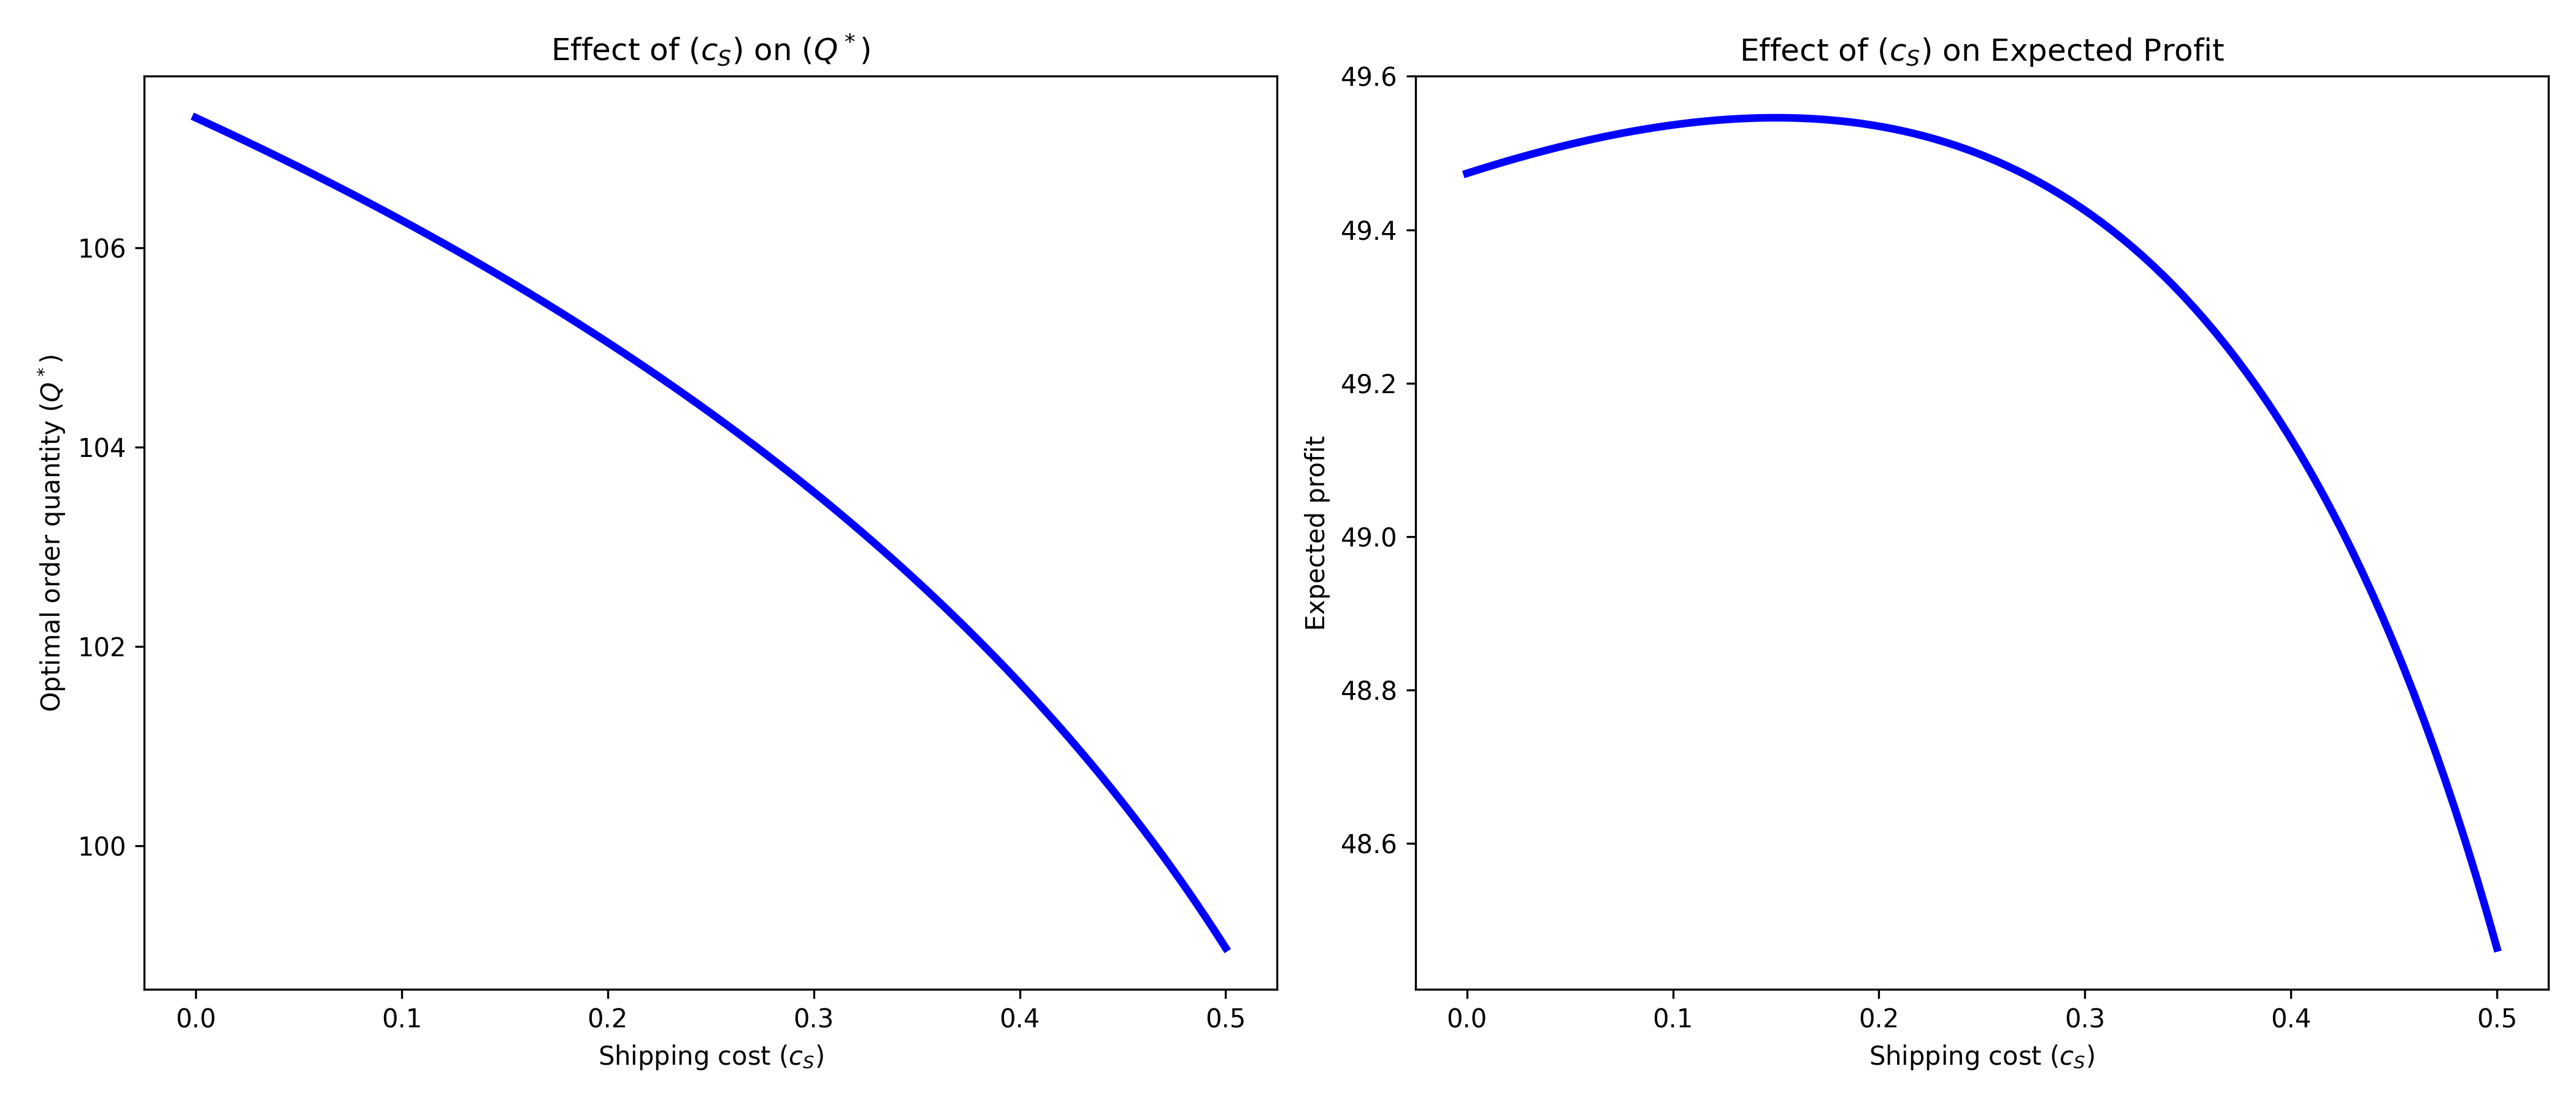
\includegraphics[width=1.00\textwidth]{figures/task2plot.png}
    \caption{Effect of shipping cost $c_S$ on optimal order quantity and expected profit}
\end{figure}


\end{document}